\documentclass{amsart}
\usepackage{graphicx}
\title{Variational approximations to zero-inflated Bayesian models}
\author{Mark Greenaway}
% include.tex
\newcommand{\Bernoulli}[1]{\text{Bernoulli} \left( #1 \right)}
\newcommand{\mydigamma}[1]{\psi \left( #1 \right)}
%\newcommand{\diag}[1]{\text{diag}\left( #1 \right)}
\newcommand{\tr}[1]{\text{tr}\left( #1 \right)}
\newcommand{\Poisson}[1]{\text{Poisson} \left( #1 \right)}
\def \half {\frac{1}{2}}
\def \R {\mathbb{R}}
\def \vbeta {\vec{\beta}}
\def \vy {\vec{y}}
\def \vmu {\vec{\mu}}
\def \vmuqbeta {\vmu_{q(\vbeta)}}
\def \vmubeta {\vmu_{\vbeta}}
\def \Sigmaqbeta {\Sigma_{q(\vbeta)}}
\def \Sigmabeta {\Sigma_{\vbeta}}
\def \va {\vec{a}}
\def \vtheta {\vec{\theta}}
\def \mX {\vec{X}}

\def\ds{{\displaystyle}}

\def\diag{{\mbox{diag}}}

\begin{document}
\maketitle
% First, simplest zero-inflated count model to consider.
Count data with a large number of zero counts arises in many areas of
application, such as data arising from physical activity studies, 
insurance claims, hospital visits or defects in manufacturing processes.

\section{A factorised variational approximation to the univariate zero-inflated Poisson model}

% TODO: Add graphical model

We use a factorised approximation to the full likelihood, as detailed in \cite{ormerod10}.
The use of conjugate priors in the full model yields easier mean field updates in the
variational approximation.

\noindent Consider $X_1, X_2, \ldots, X_n$ where $X_i = R_i Y_i$, $Y_i \sim \Poisson{\lambda}$ independent of
$R_i \text{indep.} \sim \Bernoulli{\rho}$. Let $\rho \sim \Unif{0, 1}$, 
$\lambda \sim \Gamma(a, b)$ and $r_i | \rho \sim \Bernoulli{\rho}$, $1 
\leq i \leq n$. Then the joint likelihood is:

$$
p(\vx, \vr, \lambda, \rho) = \frac{b^a \lambda^{a - 1} \exp{(-b \lambda)}}{\Gamma{(a)}} \prod_{i=1}^n \frac{\exp{(-\lambda r_i)} (\lambda r_i)^{x_i}}{x_i !} \rho^{r_i} (1 - \rho)^{1 - r_i}.
$$

\noindent We calculate the full conditionals for $\lambda$, $\rho$ and $\vr$.

\subsection{Full conditional for $\lambda$}
First, we calculate the full conditional for $\lambda$.

%\begin{align*}
%p(\lambda|\vx, \vr, \rho) &= \frac{\prod_{i=1}^n p(x_i | \lambda, r_i) p(\lambda) p(r_i|\rho) p(\rho)}{\int \prod_{i=1}^n p(x_i | \lambda, r_i) p(\lambda) p(r_i|\rho) p(\rho)) d \lambda}.
%\end{align*}
%
%Concentrating for now on the denominator in this expression, we re-arrange and collect
%like terms to obtain
%$$
%\prod_{i=1}^n \rho^r_i (1 - \rho)^{1 - r_i} \frac{r_i^{x_i}}{x_i !}
%	\int \frac{b^a \lambda^{a - 1} \exp{(-b \lambda)} \lambda^{x_i} \exp{(-\lambda r_i)}}{\Gamma{(a)}} d \lambda
%$$
%
%The integral in this expression is
%\begin{align*}
%& \int \frac{b^a \lambda^{(a + x_i) - 1} \exp{(-\lambda(b + r_i))}}{\Gamma{(a + x_i)}} d \lambda \frac{\Gamma{(a+ x_i)}}{\Gamma{(a)} b^{-x_i}} \\
%=& \frac{\Gamma{(a+ x_i)}}{\Gamma{(a)} b^{-x_i}}.
%\end{align*}
%
%Collecting the multiplicands in the integral over $\lambda$ together, we obtain
%$$
%\prod_{i=1}^n \rho^{r_i} (1 - \rho)^{1 - r_i} \frac{r_i^{x_i}}{x_i!}
%	\int \frac{b^{na + \sum_{i=1}^n x_i} \lambda^{(na + \sum_{i=1}^n x_i) - 1} \exp{(-\lambda(nb + \sum_{i=1}^n r_i))}}{\Gamma{(na + \sum_{i=1}^n x_i)}} d \lambda
%	\frac{\Gamma{(na + \sum_{i=1}^n x_i)}}{\Gamma{(na)} b^{-\sum_{i=1}^n x_i}}.
%$$

%By cancelling like terms in the numerator and denominator of the full likelihood we arrive 
%at
The functional form of the full conditional is proportional to

$$
b^{a+\sum_{i=1}^n x_i} \lambda^{(a + \sum_{i=1}^n x_i) - 1} \exp{\left(-(b + \sum_{i=1}^n r_i) \lambda \right)}
$$

\noindent which is clearly seen to be a Gamma distribution. Thus
$$
\lambda | \vx, \vr, \rho \sim \myGamma{a + \sum_{i=1}^n x_i, b + \sum_{i=1}^n r_i}.
$$

\subsection{Full conditional for $\rho$}
The terms of the log-likelihood involving $\rho$ are
%This integral on the right hand side is a Beta integral with the parameters
%$a = \sum_{i=1}^n r_i + 1$ and $b = (n - \sum_{i=1}^n r_i) + 1$. All of the terms in the %numerator and 
%denominator of the full conditional cancel except for
$$
\frac{\rho^{\sum_{i=1}^n r_i} (1 - \rho)^{n - \sum_{i=1}^n r_i}}{\Beta{\sum_{i=1}^n r_i + 1, n - \sum_{i=1}^n r_i + 1}}
$$

and thus we see that $\rho | \vx, \vr, \lambda \sim \Beta{\sum_{i=1}^n r_i + 1, (n - \sum_{i=1}^n r_i) + 1}$.

\subsection{Full conditional for $r_i$}
\begin{align*}
p(r_i | \text{rest}) \propto \frac{(\lambda r_i)^{x_i} \exp{(-\lambda r_i)}}{x_i !} \rho^{r_i} (1 - \rho)^{1 - r_i} \\
\propto r_i^{x_i} (e^{-\lambda})^{r_i} \rho^{r_i} (1 - \rho)^{1 - r_i}
\end{align*}.

We make use of the fact that if $x_i = 0$, $r_i = 0$, and if $x_i \ne 0$,
$r_i = 1$. So $x_i^{r_i} = I(x \ne 0)$ and hence the likelihood can be re-written as

\begin{align*}
p(r_i | \text{rest}) &= \frac{(e^{-\lambda + \logit{\rho}})^{r_i}}{I(x_i = 0) + (e^{-\lambda + \logit{\rho}})^{r_i}} \\
&= \Bernoulli{\text{expit}(\eta_i)}
\end{align*}.

% Step Two: Assume q(r_i) = Bernoulli(\rho_i), 1 \leq i \leq n for some known \rho_i. Find the
% variational Bayes updates of the q-densities q(\lambda) and q(\rho) corresponding to the
% factorisation
% q(\vr, \lambda, \rho) = q(\lambda) q(\rho) \sum_{i=1}^n q(r_i)

We assume a factorised approximation of the form

$$
q(\theta) = q(\lambda) q(\rho) \prod_{i=1}^n q(p_i)
$$

where $q(\lambda)$ is a Gamma distribution, $q(\rho)$ is a Beta distribution and
$q(p_i)$ are Bernoulli distributions.

%By taking the expectation of each full conditional with respect to 

\subsection{Mean field update equations}
We are now in a position to calculate the mean field update equations for the factorised
variational approximation.

Assuming that $q^*(r_i) \sim \Bernoulli{p_i}$,

\begin{align*}
q^*(\lambda) &\propto \lambda^{a+\sum_{i=1}^n x_i - 1} \exp{\left[ E_{-q(\lambda)} \{-(b + \sum_{i=1}^n r_i) \lambda \} \right]} \\
&\propto \lambda^{a+\sum_{i=1}^n x_i - 1} \exp{\{-(b + \sum_{i=1}^n p_i)\lambda \} } \\
&= \myGamma{a+\sum_{i=1}^n x_i, b + \sum_{i=1}^n p_i}
\end{align*}

and

\begin{align*}
q^*(\rho) &\propto \exp{\{ E_{-q(\rho)} \left[ \sum_{i=1}^n r_i \log{(\rho)} + \sum_{i=1}^n (1- r_i) \log{(1 - \rho)} \right] } \\
&\propto \exp{ \left( \sum_{i=1}^n p_i \log{\rho} + \sum_{i=1}^n (1 - p_i) \log{(1 - \rho)} \right) } \\
&= \Beta{1+ \sum_{i=1} p_i, n - \sum_{i=1}^n p_i + 1}
\end{align*}

Turning our attention now to $r_i$, we first note that the relevant terms of the
log-likelihood are

$$
-\lambda r_i + x_i \log{r_i} + r_i \log{\left(\frac{\rho}{1 - \rho}\right)}
$$

Taking expectations with respect to $\lambda$ and $\rho$ we have

$$
-r_i \frac{\alpha_\lambda^*}{\beta_\lambda^*} + x_i \log{(r_i)} + r_i (\Psi(\alpha_\rho^*) - \Psi(\beta_\rho^*))
$$

Note that if $x_i = 0$ then
$x_i \log{(r_i)} = \log{(x_i^{r_i})} = \log{(0^0)} = \log{(1)} = 0$. Dr John Ormerod hit
upon the idea of side-stepping this problem by writing the q-likelihood as

$$
q_{r_i}^*(r_i) \propto r_i^{x_i} \exp{(r_i \eta_i)}
$$

where $\eta_i = - \frac{\alpha_\lambda^*}{\beta_\lambda^*} + \Psi(\alpha_\rho^*) - \Psi(\beta_\rho^*)$.

Now, either $x_i = 0$ or $x_i \ne 0$.

\begin{align*}
p_i &= \frac{\exp{(\eta_i)}}{I(x_i = 0) + \exp{(\eta_i)}} \\
&= \text{expit}(\eta_i)
\end{align*}

\subsection{Lower bound}
The lower bound $\log{p(x)}$ is
$$
	E_q[\log{p(x, \theta)} - \log{q(\theta)}]
$$

where $q(\theta) = q(\lambda) q(\rho) \prod_{i=1}^n q(r_i)$,
$q(\lambda) \sim \text{Gamma}{(a_\lambda^*, b\lambda^*)}$,
$q(\rho) \sim \text{Beta}(a_\rho^*, b_\rho^*)$ and
$q(r_i) = 1$ if $x_i \ne 0$, and $p_i$ if $x_i = 0$, where $p_i$ is
calculated for each iteration as specified above.

In this case, the lower bound can be calculated directly to be

\begin{align*}
\bbE_q \left\{ \log{p(\vx, \vr, \lambda, \rho)} - \log{q(\vr, \lambda, \rho)} \right\} &= 
a \log{(b)} + (a - 1) \bbE[\log{(\lambda)}] - b \bbE [\lambda] - \log{(\Gamma(a))} \\
&+ \sum_{i=1}^n  ( -\bbE [\lambda] \bbE [r_i] + \bbE[x_i \log{(\lambda r_i)}] - \log{(x_i!)} \\
&+ \bbE[r_i] \bbE[\log{(\rho)}] + \bbE[(1 - r_i)] \bbE[\log{(1 - \rho)}] ) \\
& - \bbE \log{q(r)} - \bbE \log{q(\lambda)} - \bbE \log{q(\rho)}
\end{align*}

where
$$
\bbE [\log{\lambda}] = -\{ a_\lambda^* - \log{(b_\lambda^*)} + \log{\Gamma(a_\lambda^*)} + (1 - a_\lambda^*) \psi{(a_\lambda^*)} \} \\
$$
$$
\bbE [\lambda] = \frac{a_\lambda^*}{b_\lambda^*} \\
$$
$$
\bbE[\log{\rho}] = - \{ \log{B(a_\rho^*, b_\rho^*)} - (a_\rho^* - 1) \psi{(a_\rho^*)} - (b_\rho^* - 1)\psi{(b_\rho^*)} + (a_\rho^* + b_\rho^* - 2)\psi{(a_\rho^* + b_\rho^*)} \} \\
$$

By symmetry, we see that $(1 - \rho)$ has the same entropy as $\rho$,
and so $\bbE [\log{(\rho)}] = \bbE [\log{(1 - \rho)}]$.
$$
\bbE[r_i] = 
	\begin{cases}
	1 & \text{if } x_i \ne 0 \\
	p_i & \text{if } x_i = 0 \\
	\end{cases}
$$

$$
-\bbE_q \log{q(r)} = \sum_{i=1}^n I(x_i = 0) \log{(p_i)}
$$

$$
-\bbE_q \log{q(\lambda)} = q_q^* - \log{(b_q^*)} + \log{\Gamma{(a_q^*)}} + (1 - a_q^*) \Psi{(a_q^*)}
$$

$$
\bbE[\log{q(\rho)}] = - \{ \log{(B(a_q^*, b_q^*)} - (\alpha_q^* - 1) \psi{(a_q^*)} - (\beta_q^* - 1)\Psi{(\beta_q^*)} + (\alpha_q^* + \beta_q^* - 2)\Psi{(\alpha_q^* + \beta_q^*)} \}
$$

\subsection{Results}
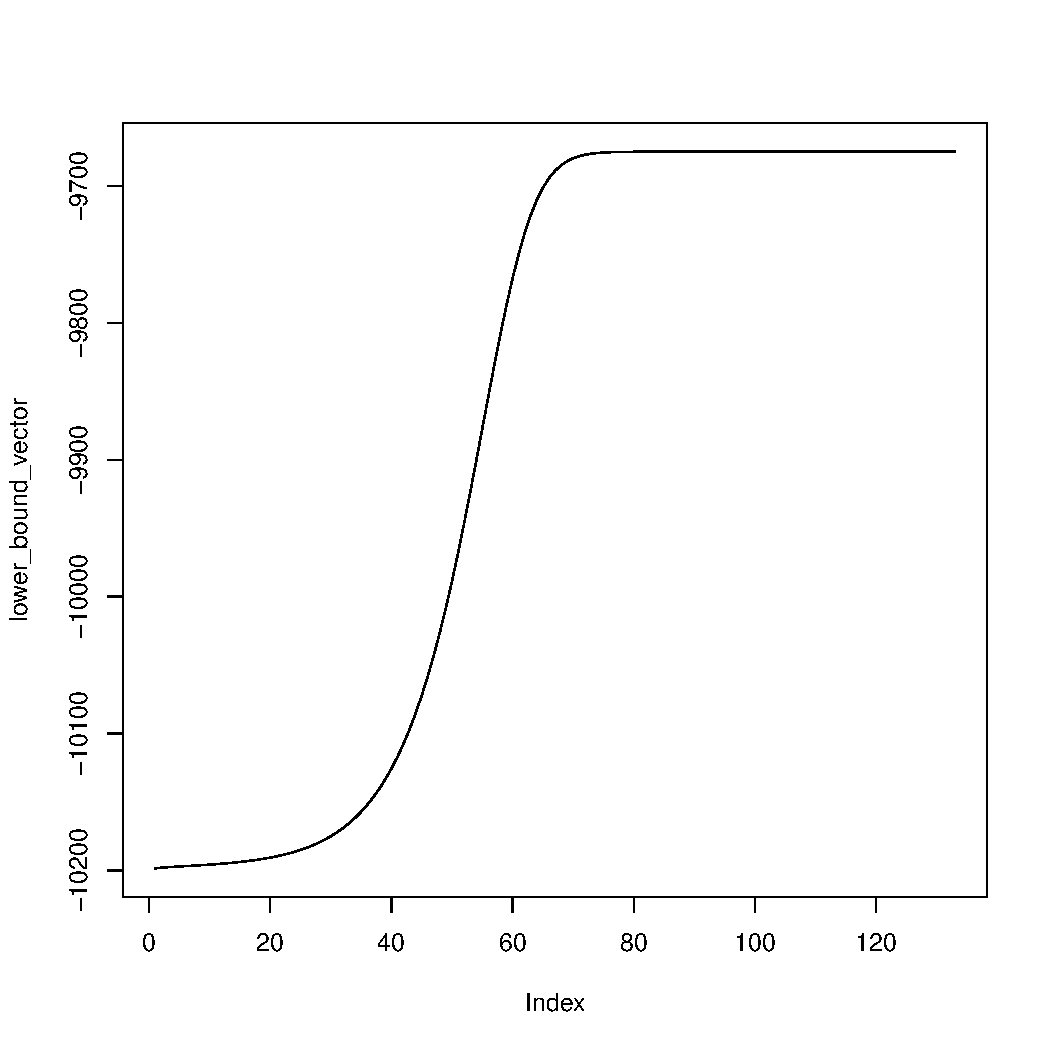
\includegraphics[width=100mm,height=100mm]{code/lower_bound_convergence.pdf}

\section{Extending the zero-inflated Poisson model to a regression model}
The above univariate model demonstrates that variational approximations are well-suited
to accelerating the fit of Bayesian zero-inflated models to data. Typically zero-inflated
models arise in applications where we wish to build multivariate models. To be able to
construct multivariate models with as much generality as possible, we specify the full
model as a General Design Bayesian Generalized Linear Mixed Model, as in \cite{zhao06}.
This allows us to incorporate within-subject correlation, measurement error, missing data
and smoothing splines in our models. We replace the $\lambda$ component of the model
in the previous section with

$$
y_i|u_i \sim \exp{z_i^T(X_i \beta+ Z_i u_i) - r_i^T \exp{X_i\beta + Z_i u_i} + 1_i^T\Gamma(y_i + 1)}, u_i \sim N(0, \Sigma)
$$

where $z_i = I(y_i = 0)y_i$. The prior on $\vbeta$ is $N(0, \Sigmabeta)$.

The use of non-conjugate multivariate normal priors for $\vbeta$ make this model less
amenable to mean field updates. Instead, we use the Gaussian Variational Approximation
approach outlined in \cite{ormerod09}.

\bibliographystyle{plain}
\bibliography{Chapter_1_zero_inflated_models}

\end{document}
